\chapter{Conclusões, Trabalhos Futuros e Cronograma}\label{cap:conclusao} 

Este capítulo abordará as conclusões dessa  proposta de mestrado referentes aos resultados do capítulo \ref{cap:resultados},  bem como uma seção de Trabalhos Futuros e  Cronograma. Na seção de Conclusão serão feitas algumas considerações finais dos resultados de cada base de dados, e logo opós, na seção de Trabalhos Futuros tem a pretenção de melhorar e expandir tudo que fora realizado  nesta pesquisa, e expor que existe uma continuidade para todo esse estudo aqui elaborado. Já no Cronograma, será criado uma tabela temporal onde esta será divida em meses e tarefas definindo os passos a serem seguidos até a conclusão da dissertação.

\section{Conclusão}\label{cond}
No capítulo \ref{cap:resultados} foi aplicado algoritmos supervisionados em algumas bases de dados a fim de provar se o problema proposto por este  trabalho foi solucionado, ou não. Uma vez conhecido o problema, foi realizado a execução de dois algoritmos supervisionados servindo de amostra para provar que era possível fazer rotulação de dados com estes algoritmos (Naive Bayes e CART), tema deste trabalho. E já identificando alguns trabalhos que já haviam feito rotulação, como \citeonline{LOPES2014}, utilizando algoritmos supervisionados, a intensão deste estudo era demonstrar de forma empírica a execução de outros algoritmos com paradigmas diferentes, aos que já foram realizados em pesquisas anteriores. 

Como o cerne da pesquisa é a rotulação de dados foi apresentados dois algoritmos com paradigmas diferentes, e em ambos, suas execuções nas bases de dados resultaram em respostas satisfatórias no âmbito da rotulação. Embora os rótulos encontrados  em cada base de dados não tenham sido totalmente idênticos, tanto um algoritmo como outro mostraram semelhanças em vários rótulos gerados, como exemplo das bases Iris e Glass.

Como já visto na subseção \ref{cap:ferramentas:ssec:rotulacao} o processo de rotulação é composto por um ou vários atributos de maior relevância entre eles junto com sua(s) faixa(s) de valor(es) que mais se repetem. Seguindo esse modelo foram adicionadas a cada resultado tabelas mostrando em porcentagem o grau de correlacionamento entre os atributos. A importância desta informação é passar o comportamento destes atributos adquirindo uma idéia geral da correlação entre eles na escolha do atributo rótulo.

No modelo de resolução proposto foi inicialmente utilizado Naive Bayes na base de dados Seeds\footnote{Seção \ref{cap:resultados:ssec:seed:nb}}. Logo o resultado do algoritmo nesta base, tabela ~\ref{tab:execucoes:seed:nb} de correlação entre os atributos, também exibido na coluna \textbf{Relevância} da tabela \ref{tab:rot:seeds:nb}. Dessa forma fica fácil identificar quais os atributos podem ser os rótulos dos clusters. Embora essa decisão possa ser modificada de acordo com o valor da variável ${V}$, variável essa criada para melhor escolher os atributos do rótulo, e podendo assumir valores diferentes dependendo do comportamento da base de dados.

Continuando com a base Seeds, após a escolha do atributo que fará parte do rótulo, o segundo passo é a escolha da faixa de valores do atributo. Essa segunda etapa é dependente totalmente da discretização\footnote{seção ~\ref{cap:refTeor:sec:discret}} e independente da primeira etapa. O método é capaz de gerar a faixa de maior repetição de valores de qualquer atributo, mas aqui neste trabalho o que importa é a faixa do atributo rótulo. Para ter mais  confiabilidade  no rótulo o método escolhe a faixa de valores que mais se repetem. No caso desse algoritmo o resultado na tabela \ref{tab:rot:seeds:nb} consegue provar uma boa eficiência, pois em cada 70 elementos do cluster 1, somente 14, ficaram de fora dessa faixa. No cluster 2, somando os dois atributos rótulos tem-se 12 elementos que não estão dentro da representatividade do rótulo. Outro valor pequeno em relação aos 70 elementos. E no cluster 3, somente 5 elementos não estão dentro da faixa considerada rótulo.


\begin{figure}[h!]
    \centering
    \subfloat[Naive Bayes]{
        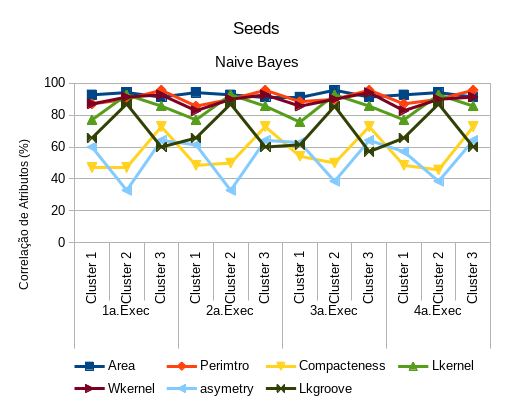
\includegraphics[scale=0.8]{figs/grafico_NB_SEED_exec_grp.png}
        \label{fig:execucoes:nb} }
    \quad
    \subfloat[CART]{
        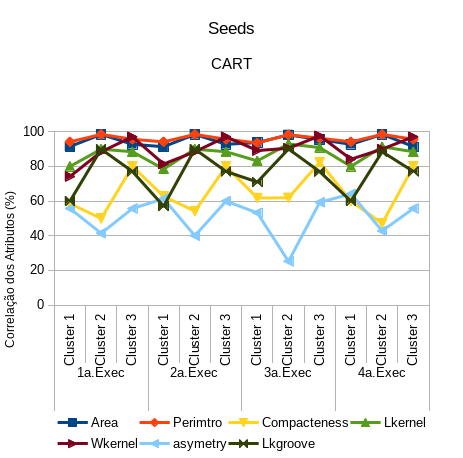
\includegraphics[scale=0.9]{figs/grafico_CART_SEED_exec_grp.png}
        \label{fig:execucoes:cart} }
    
    \caption{Gráfico de Execuções dos algoritmos supervisionados na base de dados SEEDS.} \label{fig:graf:SEED_NB_CART}
        
        %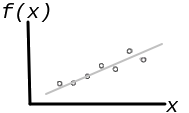
\includegraphics[scale=0.4]{figs/grafB.png}
        %\caption{Polinômio Superajustado} \label{grafB}
\end{figure}


No caso do algoritmo CART, os resultados foram diferentes dos  apresentados pelo Naive Bayes, mas nem por isso foram insatisfatórios. Contudo uma breve análise sobre as execuções das tabelas ~\ref{tab:execucoes:seed:nb} e \ref{tab:execucoes:seed:cart} podem ser observadas nos gráficos da figura ~\ref{fig:graf:SEED_NB_CART}. Como já comentado anteriormente o comportamento dos valores do correlacionamento dos atributos ao longo das execuções mostra-se equilibrada, figura ~\ref{fig:execucoes:cart}. O gráfico do CART tem um movimento semelhante ao do aplicado do Naive Bayes ~\ref{fig:execucoes:nb}, embora a variável \textbf{asymetry} saia um pouco do padrão, mas como seus valores são baixos, nada alterou nos rótulos, contudo  o valor de \textbf{perimetro} ficou bastante encostado ao valor da \textbf{area}, fazendo o rótulo \textbf{perimetro} aparecer nos grupos 1 e 2. E também só não foi escolhido pelo grupo 3 , pois  a variável \textbf{Wkernel} estava com valor mais alto. E no gráfico percebe-se que  \textbf{Wkernel} mantém valores altos em todas as execuções do grupo 3.

De acordo com o exposto acima pode-se dizer nesta análise, que o Naive Bayes acabou tendo resultados um pouco melhores, pois no que diz respeito ao número de elementos fora da faixa definida pelo rótulo, o CART, acabou por ter mais elementos fora da faixa de rótulo, comparando com os resultados do Naive Bayes. Quer dizer, o rótulo deixa de representar mais elementos usando o CART ao invés do Naive Bayes, ou em outras palavras, o Naive Bayes representou mais elementos que o CART.


\begin{figure}[h!]
    \centering
    \subfloat[Naive Bayes]{
        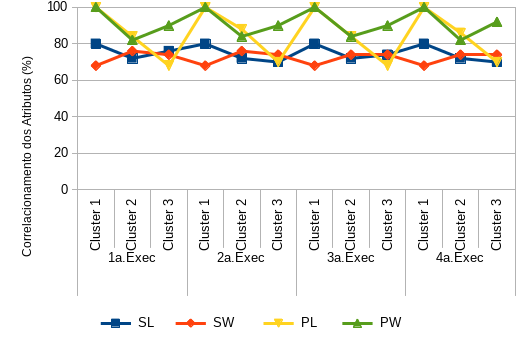
\includegraphics[scale=0.8]{figs/grafico_NB_IRIS_exec_grp.png}
        \label{fig:graf:IRIS_NB} }
    \quad
    \subfloat[CART]{
        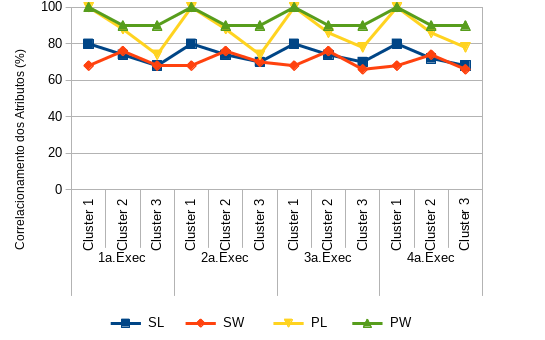
\includegraphics[scale=0.9]{figs/grafico_CART_IRIS_exec_grp.png}
        \label{fig:graf:IRIS_CART} }
    
    \caption{Gráfico de Execuções dos algoritmos supervisionados na base de dados IRIS.} \label{fig:graf:IRIS_NB_CART}
        
        %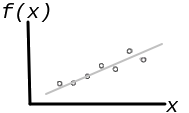
\includegraphics[scale=0.4]{figs/grafB.png}
        %\caption{Polinômio Superajustado} \label{grafB}
\end{figure}

Ja na base de dados Iris, os dois algoritmos supervisionados testados apresentaram os mesmos rótulos. Mantendo as mesmas  configurações, ${R=3}$, ${V=3\%}$ e EFD na discretização. Nos gráficos da figura ~\ref{fig:graf:IRIS_NB_CART} pode-se acompanhar como os valores dos atributos se comportam em seus clusters nas 4 iterações.

Nesta base Iris os algoritmos tem resultados nos gráficos, bastantes semelhantes, e logo se percebe que essa base contém características que possuem mais coerência com  a classe em relação ao da base SEEDS, pois nenhum atributo possui valor abaixo da linha 65(\%) de relacionamento entre eles. Embora no gráfico as  linhas referentes aos comportamentos dos atributos não sejam totalmentes iguais em cada algoritmo executado, não chegou a um valor que diferenciasse  para modificar o resultado dos rótulos como resposta.

Na rotulação encontrada pelo dois algoritmos nos resultados da tabela \ref{tab:rot:iris:nb} e \ref{tab:rot:iris:cart} o rótulo escolhido no cluster 1 teve dois atributos, \textbf{petallength} e \textbf{petalwidth} e cada um deles definiram uma faixa onde foi possível abranger 100\% de elementos dentro das faixas escolhidas por cada um dos atributos. Já no cluster 2 os mesmos atributos são escolhidos mas com faixas de valores diferentes. Embora não tivesse fechado os mesmos valores do cluster 1, obteve um total, de 7 elementos do \textbf{petallength} e 8 do \textbf{petalwidth}, totalizando 15 elementos que não estão dentro da faixa delimitada pelos rótulos. O cluster 2 possui um total de 50 elementos e 15 deles não são representados pelo rótulo do cluster. E no cluster 3 o atributo escolhido para compor o rótulo é mais uma vez o \textbf{petalwidth}. Logo se percebe a importância do atributo nos clusters, mas em nenhum deles a faixa é a mesma. Isso define bem o rótulo do cluster 3, pois o rótulo representa 45 elementos dentro do cluster, possuindo somente 5 elementos fora dessa faixa representada pelo atributo.

A repetição do atributo \textbf{petalwidth} em todos os rótulos, acaba mostrando o grau de relevância desse atributo na base de dados. Para um especialista é interessante saber que esse atributo possue um grande referencial na base de dados. Nos rótulos esse atributo assumiu faixas diferentes conseguindo assim o método da um significado ao cluster. 

Com uma breve  análise já se constata que os resultados nos dois algoritmos supervisionados foram bem satisfatórios nas bases utilizadas, conforme figura \ref{fig:graf:grafico_NB_CART_acuracia}, e  provando que é possível a rotulação de dados além de conseguir representar bem os clusters através dos rótulos encontrados. E uma obsevação técnica dos algoritmos utilizados é que o CART se mostrou bem mais rápido em relação ao Naive Bayes para gerar os resultados.

\begin{figure}[h!]
    \centering
  %  \subfloat[Naive Bayes]{
  %      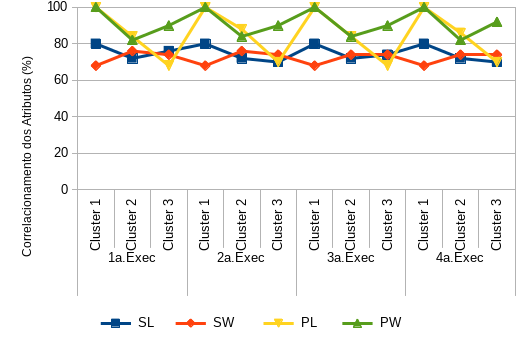
\includegraphics[scale=0.8]{figs/grafico_NB_IRIS_exec_grp.png}
  %      \label{fig:graf:IRIS_NB} }
  %  \quad
  %  \subfloat[CART]{
  %      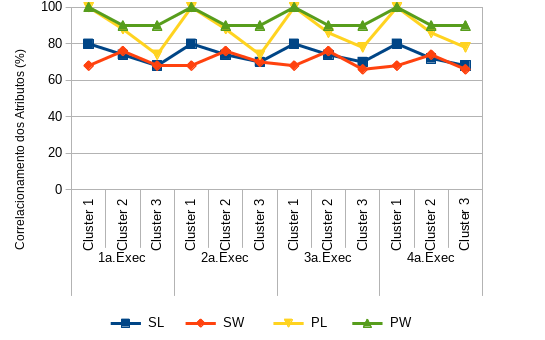
\includegraphics[scale=0.9]{figs/grafico_CART_IRIS_exec_grp.png}
  %      \label{fig:graf:IRIS_CART} }
  %  
  %  \caption{Gráfico de Execuções dos algoritmos supervisionados na base de dados IRIS.} \label{fig:graf:IRIS_NB_CART}
        
  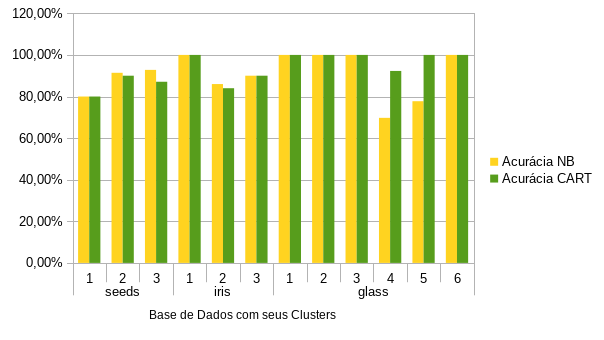
\includegraphics[scale=0.9]{figs/grafico_NB_CART_acuracia.png}
  \caption{Acurácia por Clusters} \label{fig:graf:grafico_NB_CART_acuracia}
\end{figure}





%\section*{Trabalhos Futuros}
%\addcontentsline{toc}{chapter}{Trabalhos Futuros}
\section{Trabalhos Futuros}\label{cap:fut}

A pesquisa ainda precisa de mais divulgação na esfera acadêmica, e para isso a plublicação de um artigo sobre os resultados apresentados aqui é uma consolidação dessa proposta de mestrado já voltada para a dissertação propriamente dita.

Fazer testes com mais bases de dados  e com isso traçar uma estratégia caso seja necessário a utilização da idéia de rotulação por algum fim. Caso algum órgão/setor/empresa precise utilizar a rotulação em seu meio, seria interessante o analista de dados,  saber com quais algoritmos supervisionados ele obteria melhores resultados. Embora se saiba nesse estudo que quaisquer algoritmos supervisionados são capazes de realizar a rotulação de dados, também foi provado que em algumas bases um algoritmo se sobressai a outro. Por consequencia disso ter um maior número de base com características diferentes ajudaria em uma tomada de decisão.

Outro ponto importante é inserir nos teste mais algoritmos, que pertençam a  paradigmas diferentes dos que ainda não foram utilizados. * de acordo com autor PEARSON, onde os paradigmas são divididos em :  ...... pode-se perceber que existe uma proximidade na afirmação de rotulação para quaisquer algoritmo supervisionado, não sendo ainda possível afirmar esse tema, por falta de testes em alguns algoritmos de paradigmas ainda não testados, mas já deixando par atrabalhos futuros



%\section*{Cronograma}
%\addcontentsline{toc}{chapter}{Cronograma}
\section{Cronograma}\label{cap:cron}

\definecolor{midgray}{gray}{.8}
\begin{table}[!htbp]
\caption{Cronograma de atividades}     % mude aqui para seu título da tabela
\begin{center}

% %  \resizebox{\textwidth}{!}{ % abre resizebox, setar tabela da largura da página.

\scalebox{1}{
\begin{tabular}{p{4cm}lllccc}
\hline
\multicolumn{1}{c}{\multirow{2}{*}{Atividades}} & \multicolumn{6}{c}{Meses} \\ \cline{2-7}
\multicolumn{1}{c}{} & Março & Abril & Maio & Junho & Julho & Agosto  \\ \hline \hline
%\rowcolor[HTML]{EFEFEF}
\footnotesize
Testes com Novas Bases de Dados  & \cellcolor{midgray}  ~~~~~~~~~ & \cellcolor{midgray} ~~~~~~~~~ & ~~~~~~~~~ & ~~~~~~~~~ & ~~~~~~~~~ & ~~~~~~~~~ \\ \hline
\footnotesize Modificar Números de Faixa (R) & \cellcolor{midgray}  ~~~~~~~~~ & \cellcolor{midgray} ~~~~~~~~~ &  ~~~~~~~~~ &~~~~~~~~~ & ~~~~~~~~~ & ~~~~~~~~~  \\ \hline
\footnotesize Testar com outros Métodos de Discretização     & \cellcolor{midgray}~~~~~~~~~ & \cellcolor{midgray}  ~~~~~~~~~ & ~~~~~~~~~ & ~~~~~~~~~ & ~~~~~~~~~ & ~~~~~~~~~   \\ \hline
\footnotesize Testar com outros Algoritmos com Paradigmas Diferentes & ~~~~~~~~~  & \cellcolor{midgray} ~~~~~~~~~ & \cellcolor{midgray} ~~~~~~~~~ & ~~~~~~~~~ & ~~~~~~~~~ & ~~~~~~~~~   \\ \hline
\footnotesize Preparar Artigo   & ~~~~~~~~~ & ~~~~~~~~~ & ~~~~~~~~~ & \cellcolor{midgray} ~~~~~~~~~ & \cellcolor{midgray}  ~~~~~~~~~ & ~~~~~~~~~   \\ \hline
\footnotesize Escrita da Dissertação & ~~~~~~~~~  & ~~~~~~~~~ & ~~~~~~~~~ & \cellcolor{midgray} ~~~~~~~~~ & \cellcolor{midgray} ~~~~~~~~~ & \cellcolor{midgray} ~~~~~~~~~   \\ 
\hline
\end{tabular}
} % fecha resizebox
\end{center}
\label{cronograma} % para referencia no texto.
\end{table}


